% sec_gas.tex
\section{Проверка соотношений через газокинетический метод}

В порядке косвенной оценки истинности полученных результатов используем их в существующих теоретических методах и физических моделях изучения газообразной фазы существования вещества. Используем для этого классический подход, применяемый для вывода зависимости среднего значения длины свободного пробега молекулы газа от его параметров, изложенный в «Курсе общей физики» И.В. Савельева (Т.1, Механика, колебания и волны, молекулярная физика). Надо отметить, что «псевдожидкий» Свободный эфир и газ имеют существенные структурные различия; однако общий методологический подход к решению задачи справедлив в обоих случаях, так как не требует привлечения оценки «малости» размера молекулы относительно длины её свободного пробега, поэтому понятие «эффективное сечение молекулы» может быть применено и к частице эфира-Амеру, из чего следует, что эффективное сечение Амера \(\sigma = \pi d_a^2\). Полагая скорость частицы равной среднему значению \(\|\mathbf{v}_{\text{сэ}}\|\), определим длину пути, пройденную ею за единицу времени: \(l = t \|\mathbf{v}_{\text{сэ}}\| = \|\mathbf{v}_{\text{сэ}}\|\), при этом цилиндрический объём \(V = \sigma l = \pi \|\mathbf{v}_{\text{сэ}}\| d_a^2\) включает в себя все акты соударений за указанный отрезок времени (единицу времени), и их количество равно частоте столкновений. Она может быть найдена как произведение \(\nu = V n_{\text{сэ}}\), где \(n_{\text{сэ}}\) — концентрация частиц Свободного эфира, полученная ранее на основании гипотезы \textbf{Иоганна Кеплера}, или
\[
\nu = V n_{\text{сэ}} = \frac{8\sqrt{2}}{27} \pi d_a \|\mathbf{v}_{\text{сэ}}\|.
\]
Полученное выражение не вполне соответствует действительности, так как должно включать относительные скорости соударяющихся частиц, которые в \(\sqrt{2}\) раз больше, чем \(\|\mathbf{v}_{\text{сэ}}\|\), поэтому
\[
\nu = \frac{16\pi}{27 d_a} \|\mathbf{v}_{\text{сэ}}\|.
\]
Отношение длины пройденного пути за единицу времени к частоте соударений Амеров даёт искомую величину среднего значения длины свободного пробега частицы в свободном эфире:
\[
\langle\lambda_{\text{сэ}}\rangle = \frac{l}{\nu} = \frac{\|\mathbf{v}_{\text{сэ}}\|}{ \frac{16\pi}{27 d_a} \|\mathbf{v}_{\text{сэ}}\| } = 0.5371\,d_a \approx \frac{d_a}{2}.
\]
Как видно, результат практически совпал со значением длины свободного пробега, ранее полученным из соображений целостности вихревых эфирных объектов.

Изотропность Свободного эфира, или физического вакуума, позволяет предположить неизменность концентраций частиц на единице длины произвольно выбранного направления и на единице площади произвольной поверхности, в том числе плоской, \(n_{al}\) и \(n_{as}\) соответственно. Иначе говоря, \(n_{\text{сэ}} = n_{al}^3 = n_{as} n_{al}\). Таким образом,
\[
n_{as} = n_{\text{сэ}}^{2/3} = \left(\frac{16}{27\sqrt{2}\,d_a^3}\right)^{2/3} \approx \frac{1.78}{d_a^2}.
\]
Зная концентрацию Амеров в Свободном эфире, можно оценить часть «пространства обитания» одной частицы \(V_{\text{об}}\), имея в виду, что длина её свободного пробега \(\lambda_{\text{сэ}} < d_a\):
\[
V_{\text{об}} = \frac{1}{n_{\text{сэ}}} = \frac{27\sqrt{2}}{16} d_a^3 \approx 2.4\,d_a^3.
\]
При этом объём Амера \(V_a = \frac{\pi}{6}d_a^3 \approx 0.52\,d_a^3\). На рис. \ref{fig:habitat} в качестве наглядной демонстрации изображён фрагмент гипотетически регулярной компоновки частиц эфира в «пространстве обитания». Пример показывает чрезвычайно ограниченные возможности частиц эфира совершать какие-либо существенные перемещения в пространстве в условиях хаотических столкновений.

\begin{figure}[h]
\centering
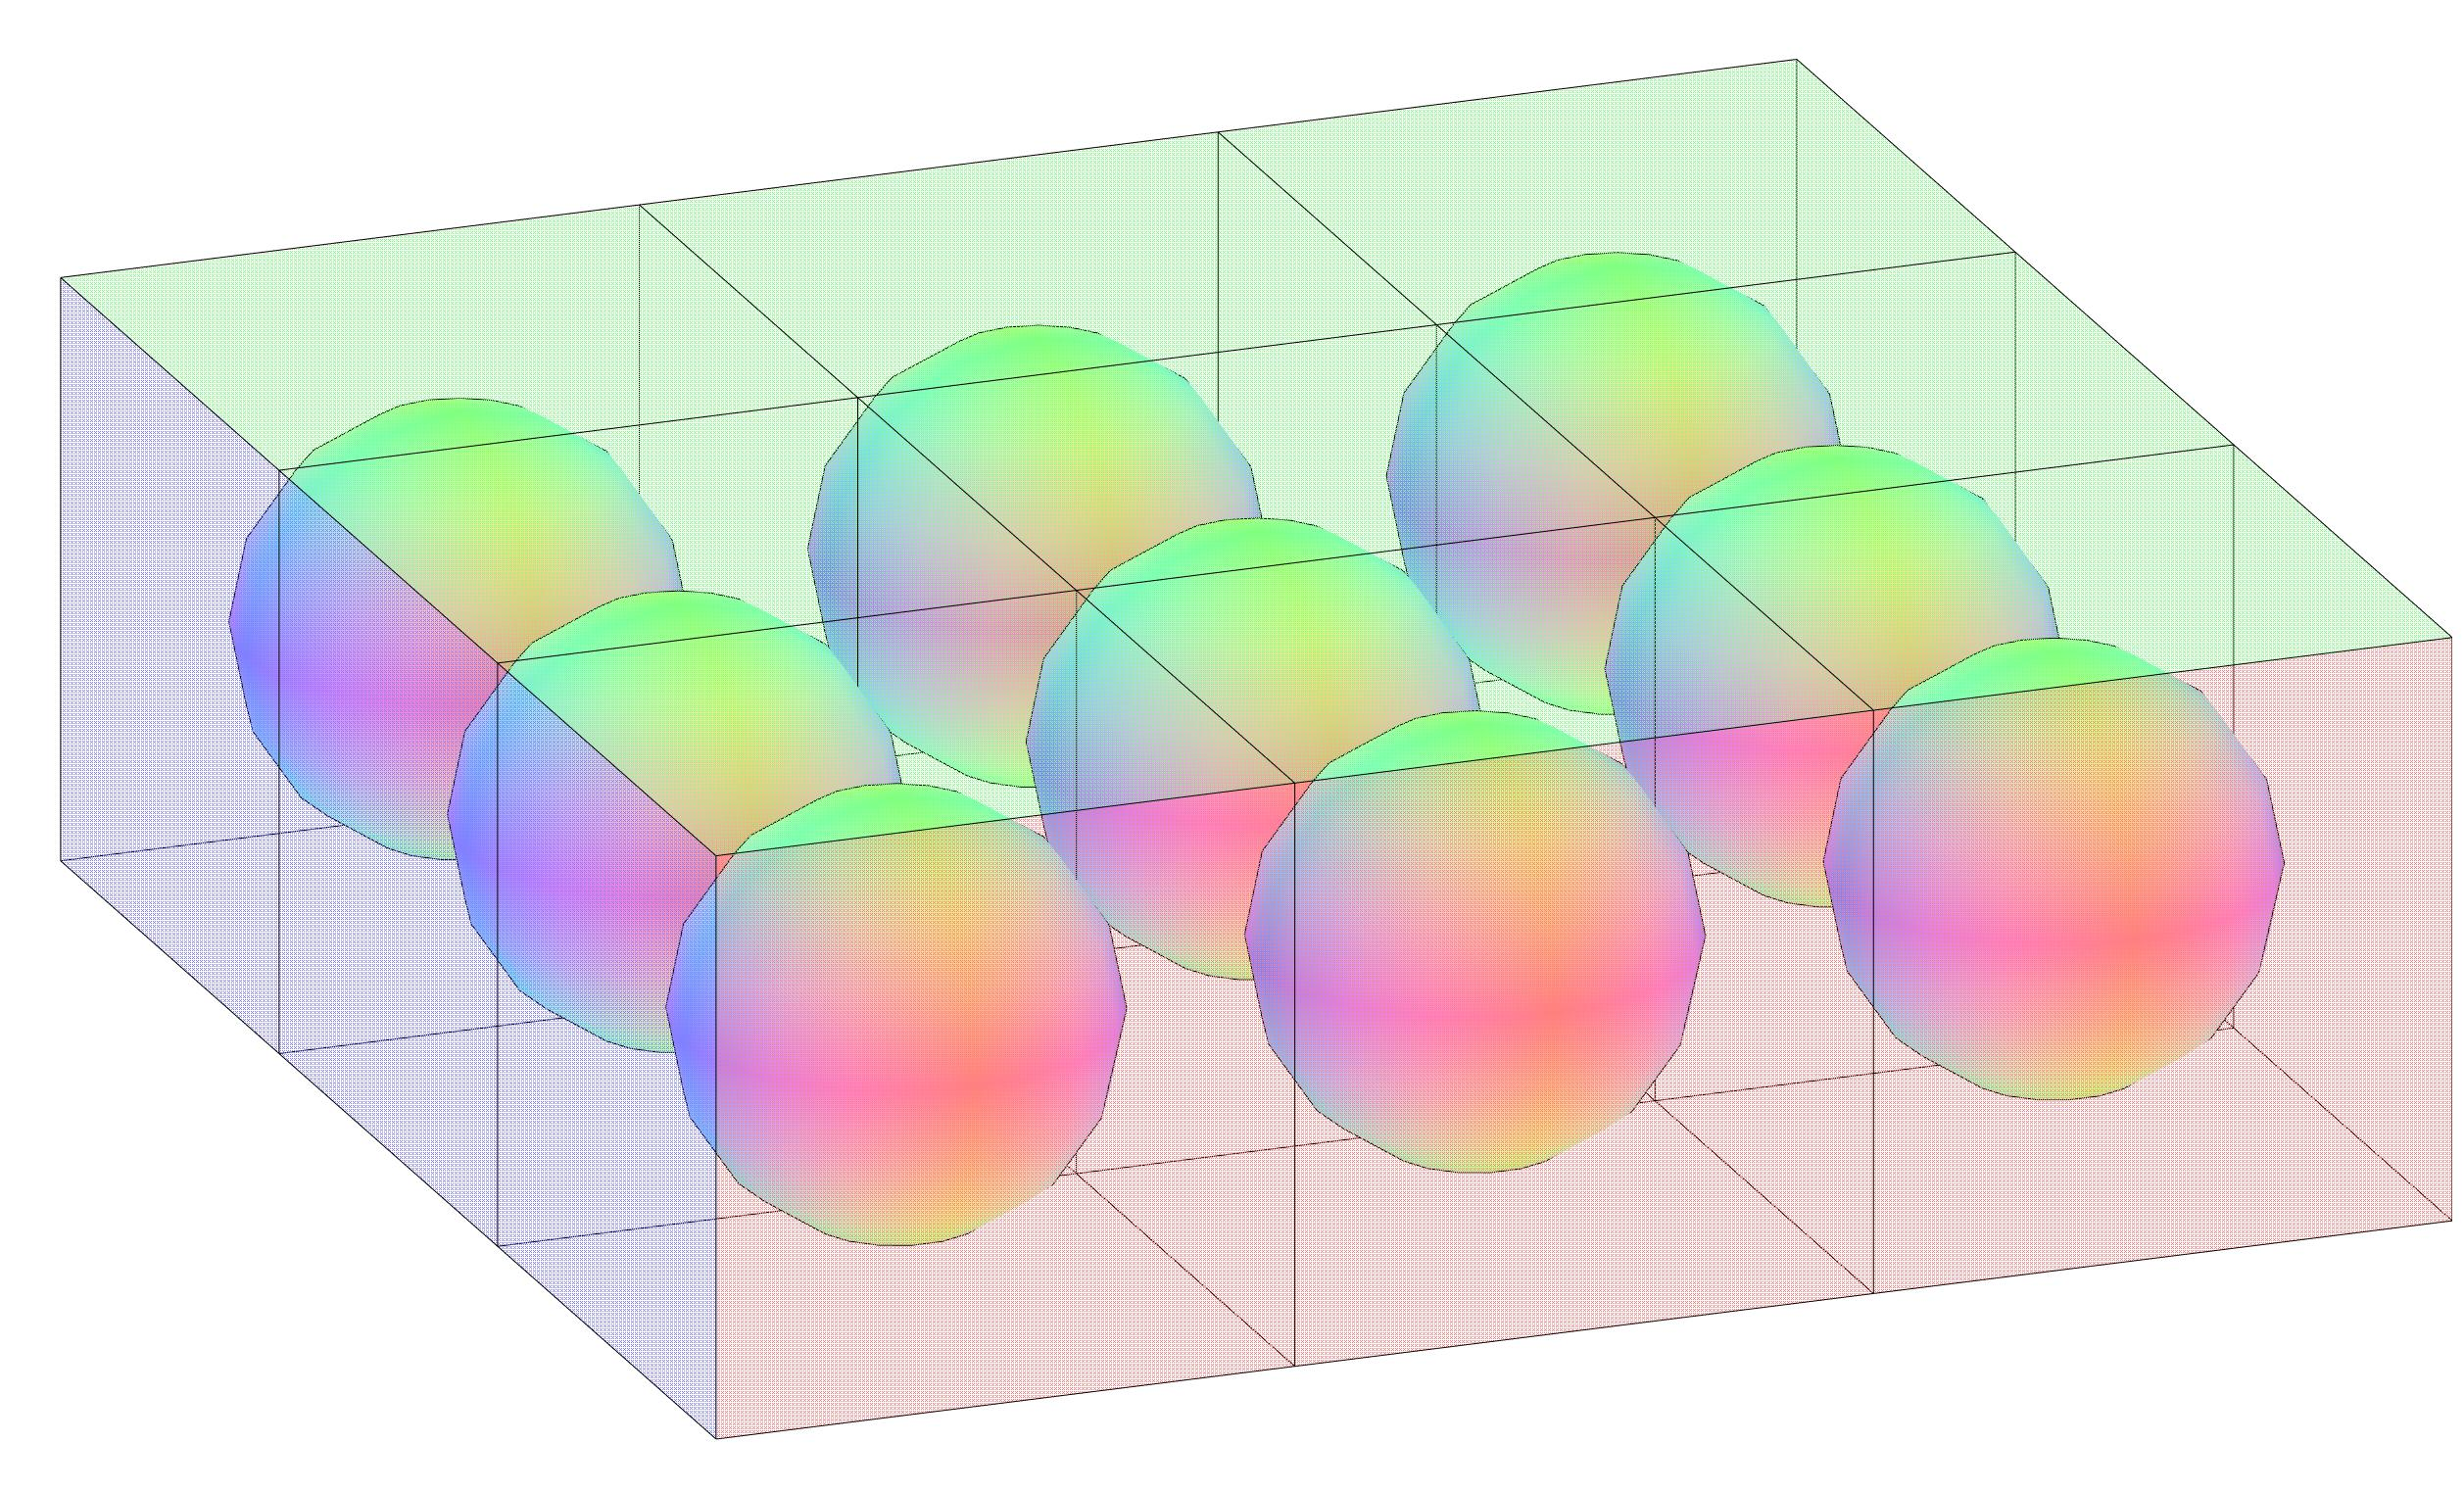
\includegraphics[width=0.3\textwidth]{images/a28.png}
\caption{«Пространство обитания» Амера в СЭ.}
\label{fig:habitat}
\end{figure}

На рис. \ref{fig:random1} и \ref{fig:random2} изображён пространственно-временной фрагмент случайного (стохастического) распределения Амеров свободного эфира.

\begin{figure}[h]
\centering
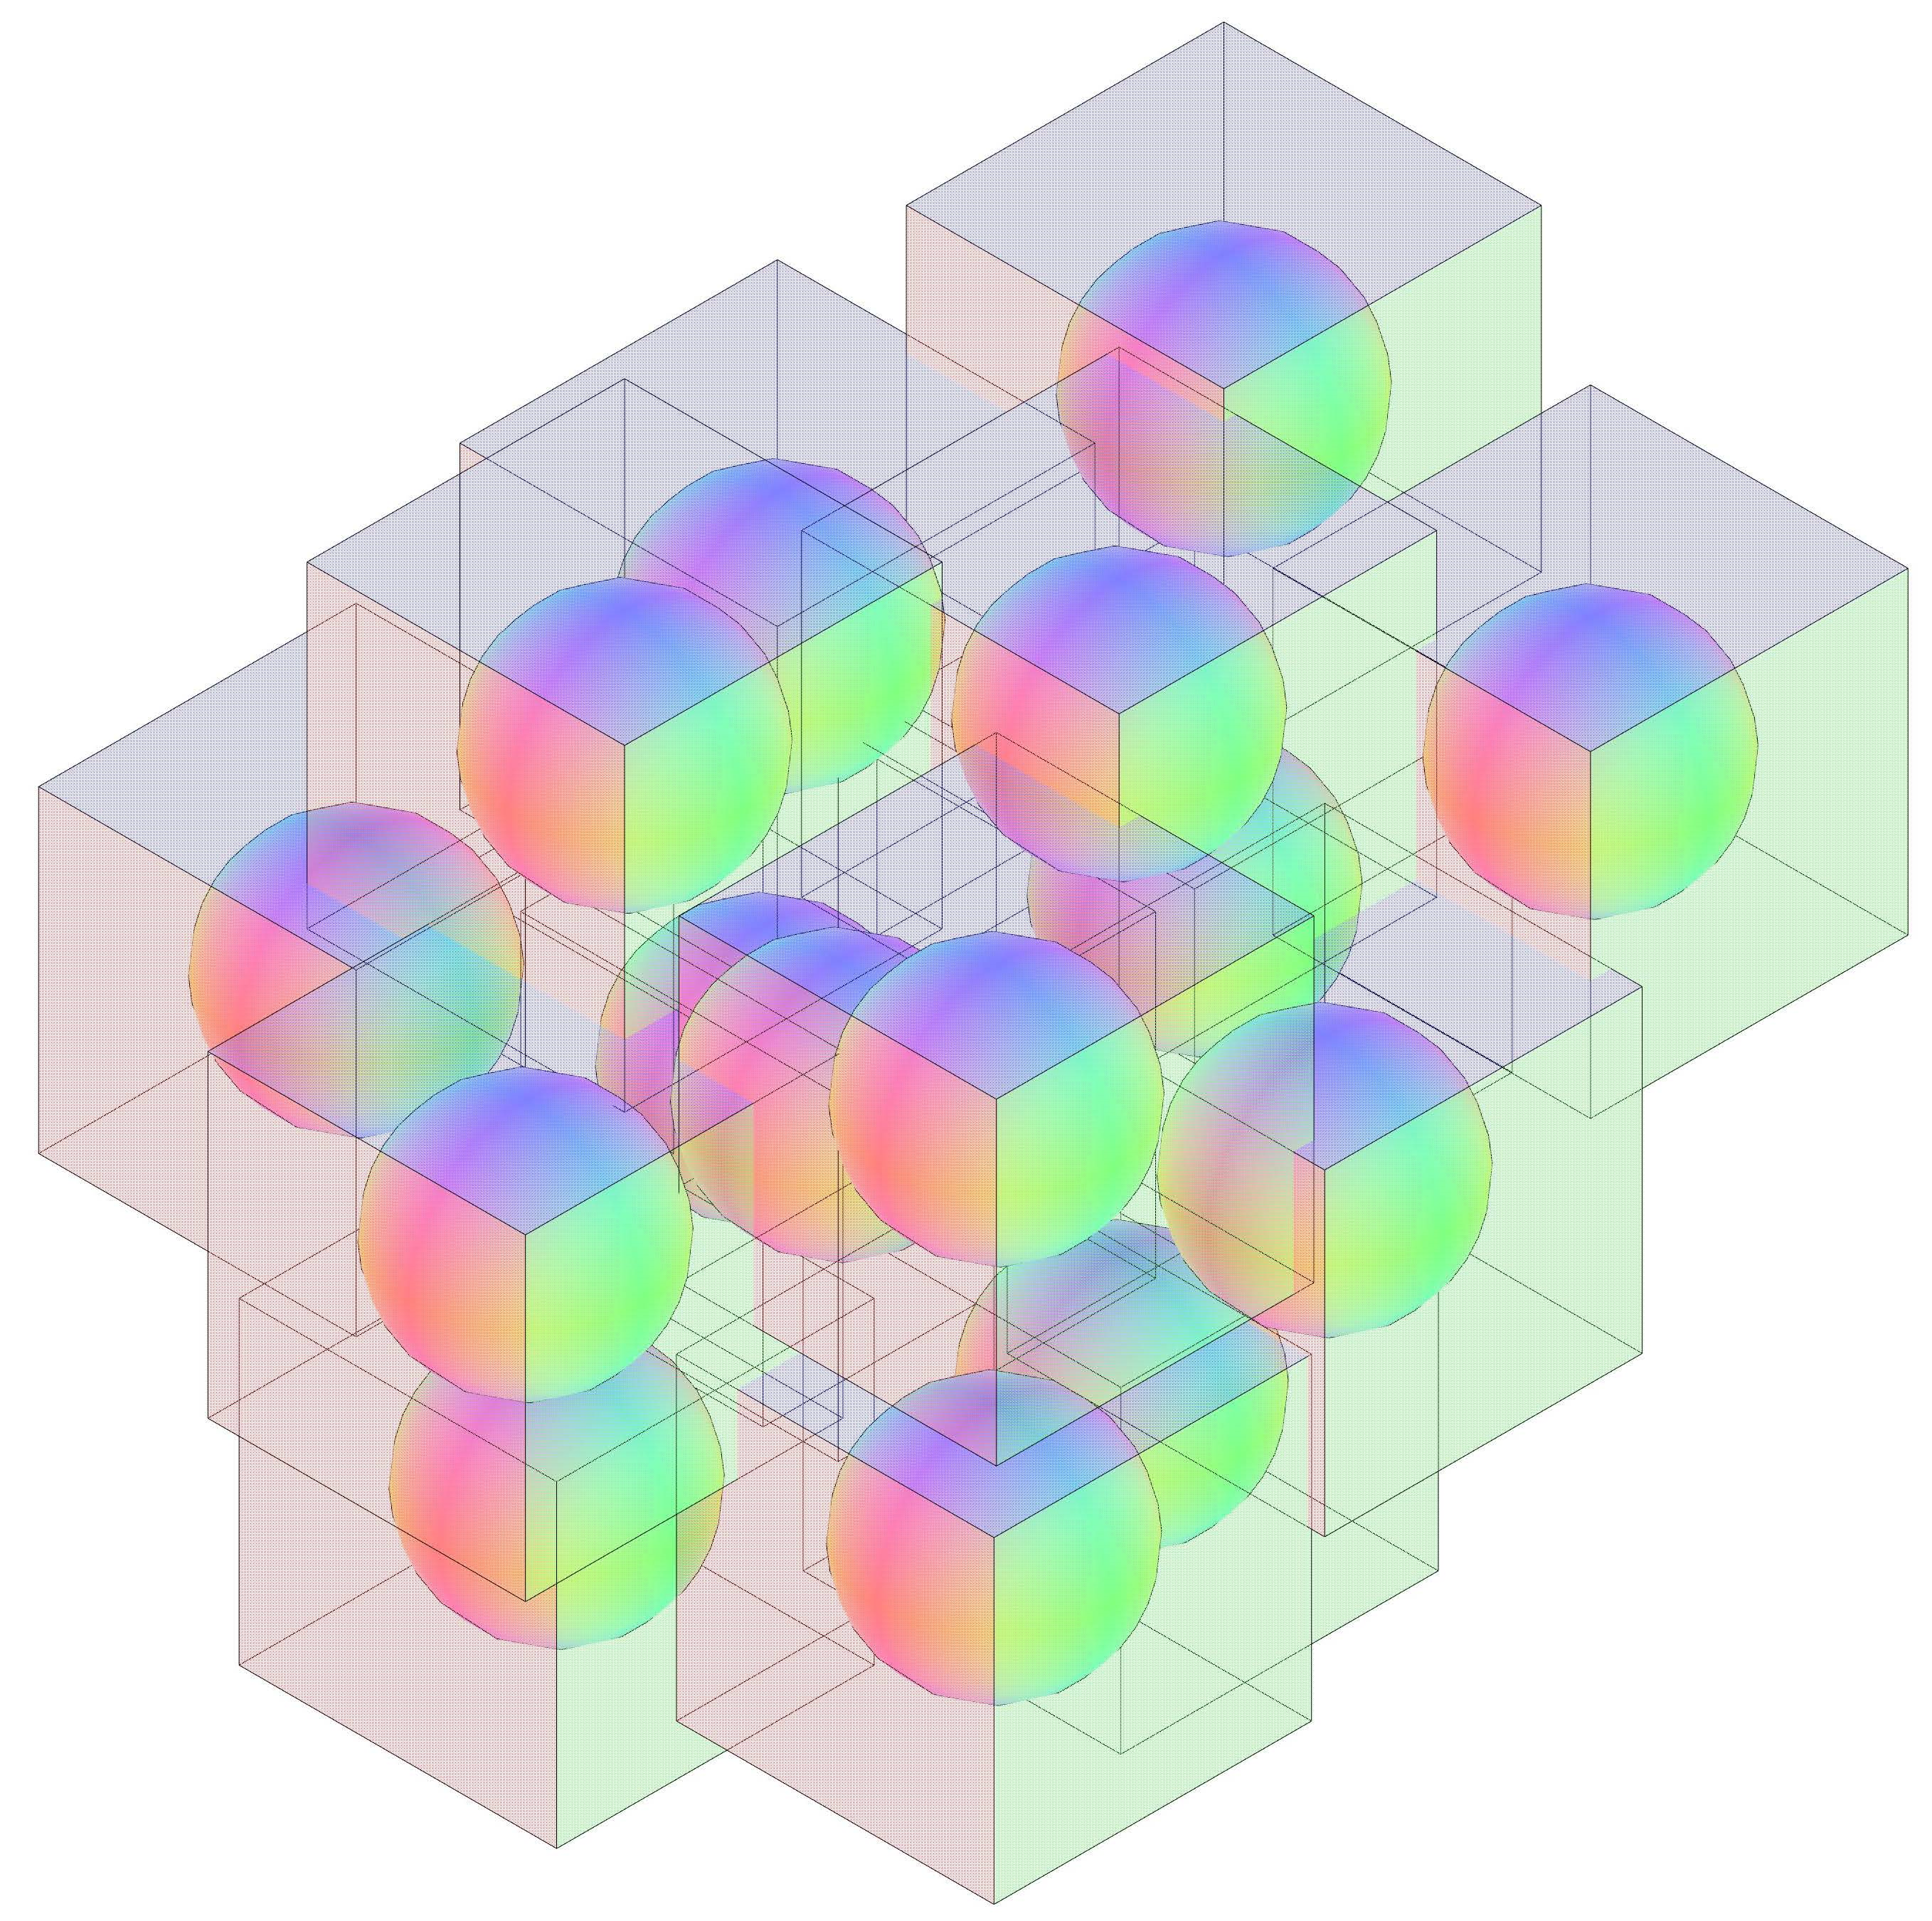
\includegraphics[width=0.3\textwidth]{images/a23.png}
\caption{Фрагмент нерегулярной упаковки СЭ.}
\label{fig:random1}
\end{figure}

\begin{figure}[h]
\centering
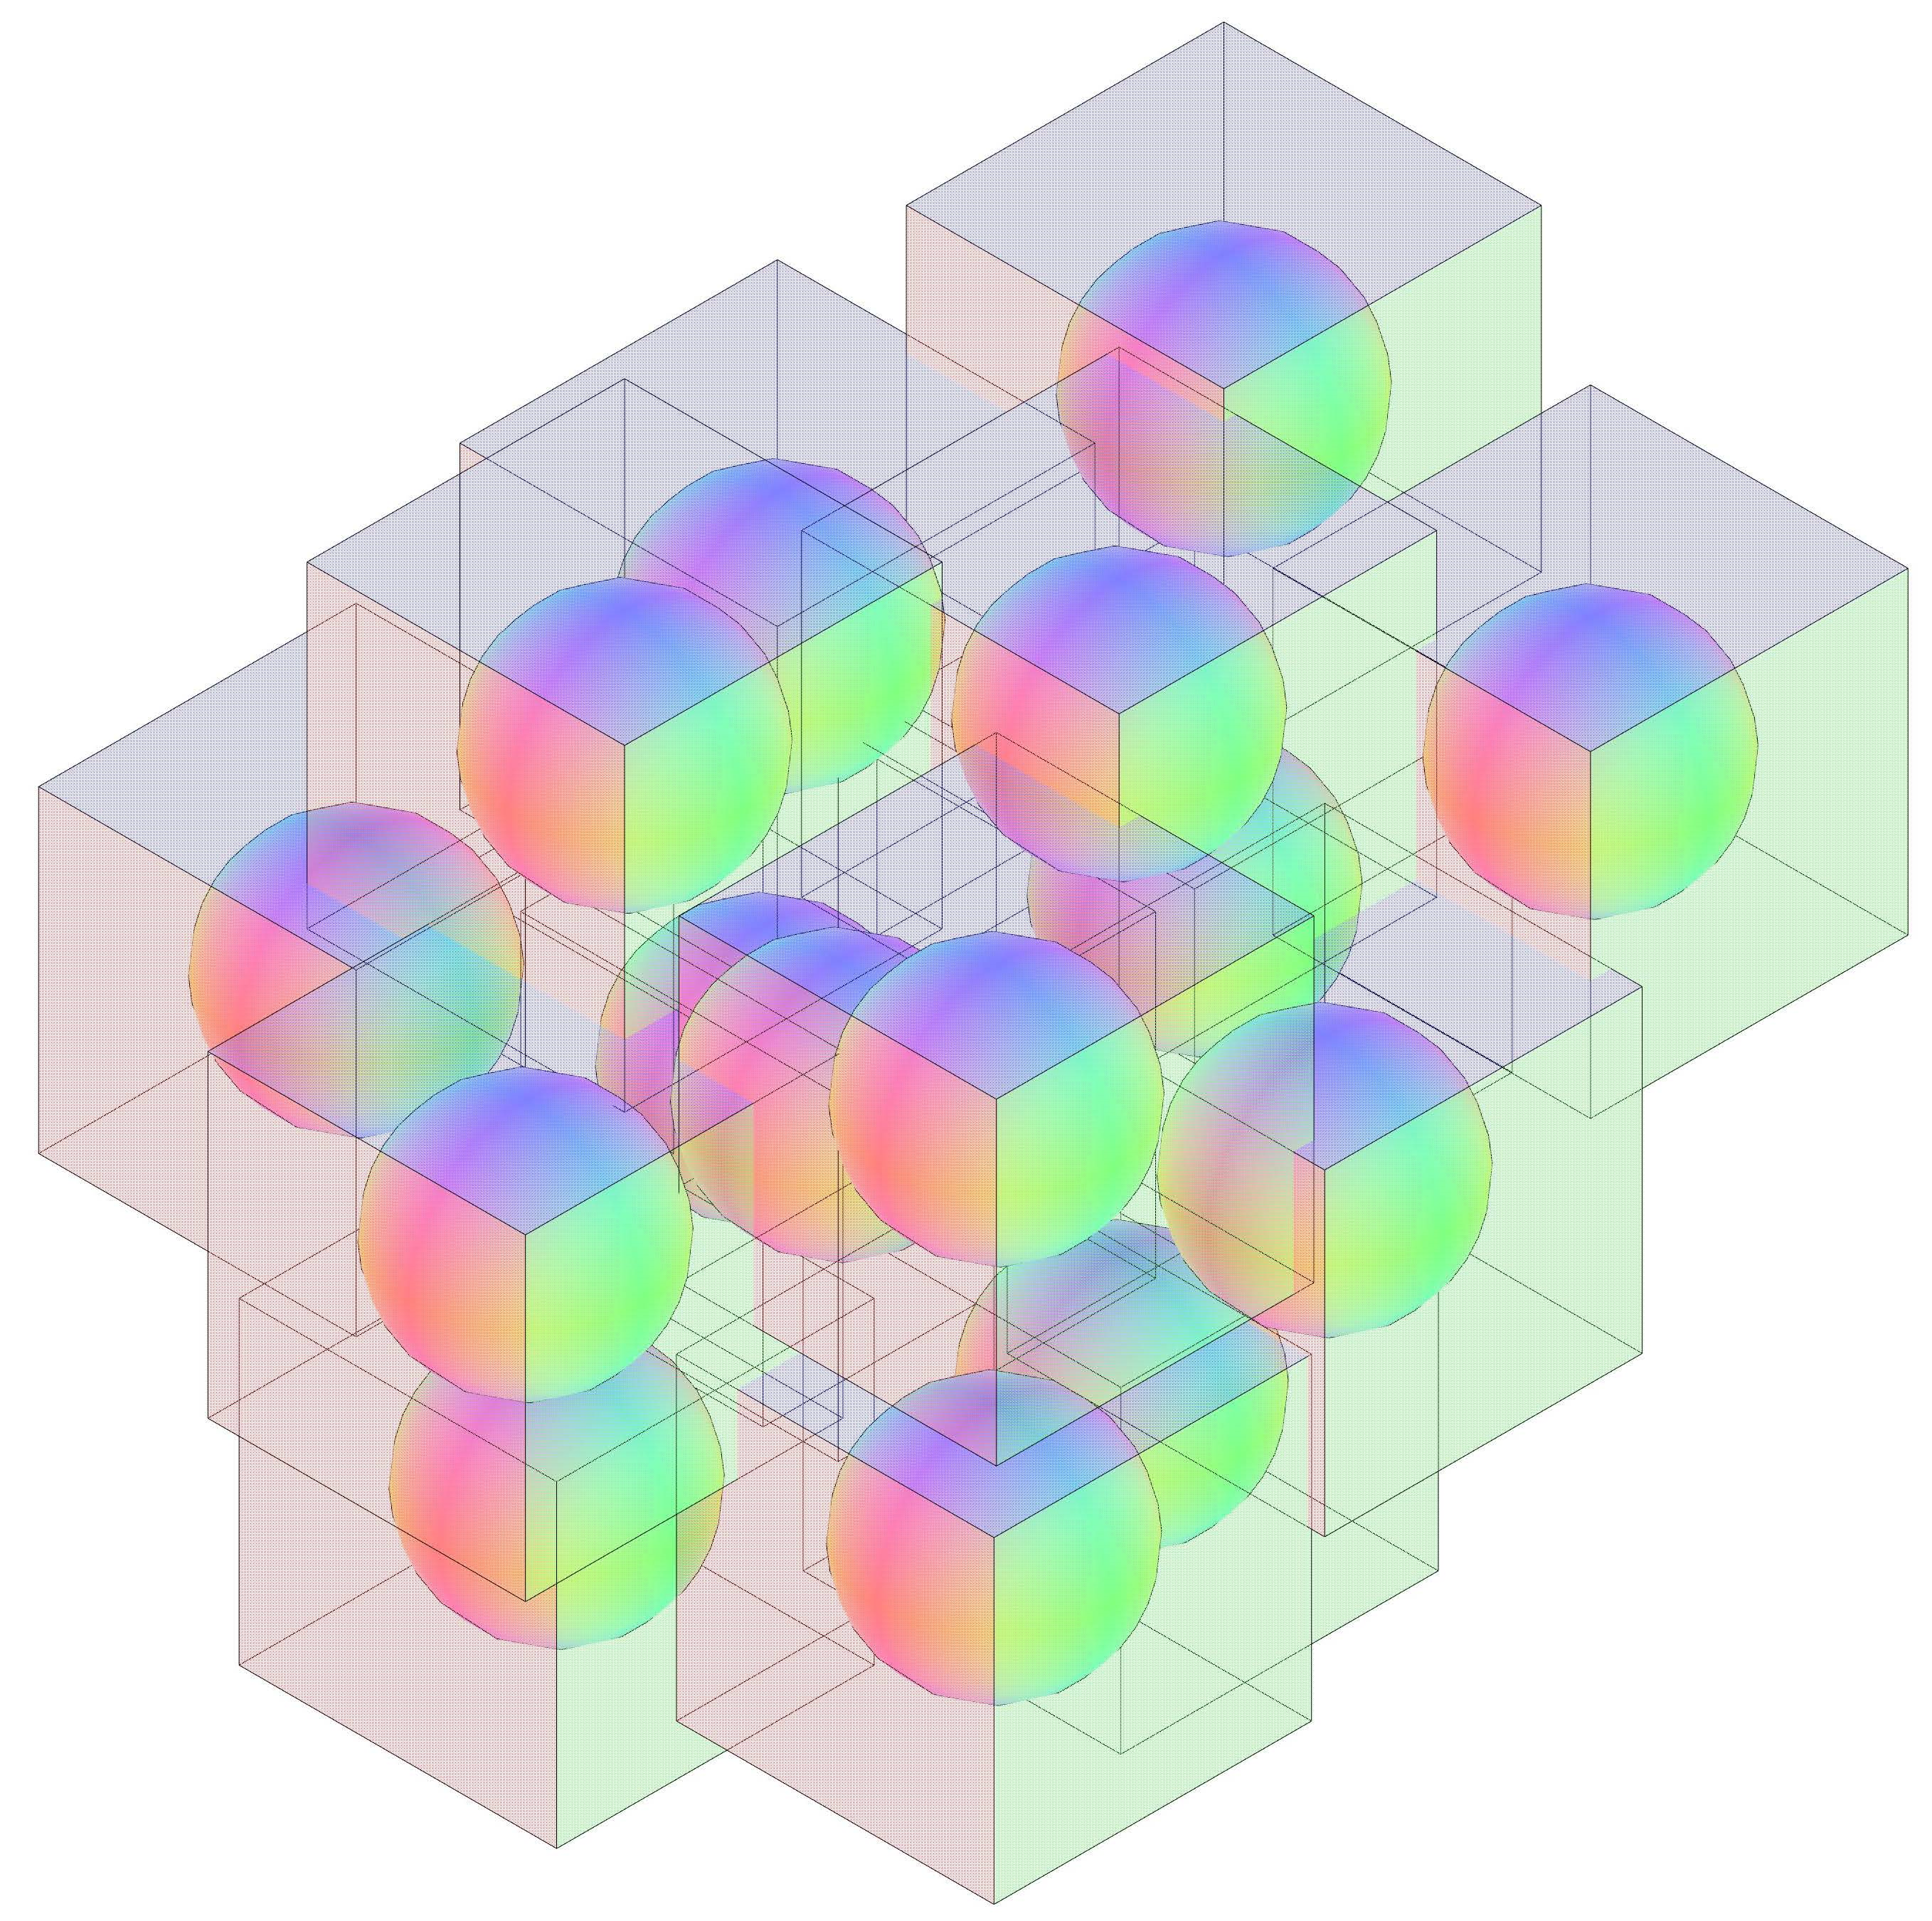
\includegraphics[width=0.3\textwidth]{images/a23.png}
\caption{Фрагмент упаковки СЭ.}
\label{fig:random2}
\end{figure}

Величина перемещения частицы в результате последовательности соударений в случае Свободного эфира является случайной величиной и относится к нормальному распределению плотности вероятности Гаусса–Лапласа. Идеальный характер столкновений и \(\langle\lambda_{\text{сэ}}\rangle \approx d_a/2\) указывают на то, что вероятность перемещения частицы между парой соударений на расстояние, близкое по величине \(d_a/2\), наибольшая. Следствием этого является «пространственная привязанность» или «оседлость» частиц Свободного эфира. Миграция Амеров безусловно возможна, но этот процесс — событие с малой долей вероятности, и на настоящем этапе исследований его влиянием можно пренебречь.

Пренебрежительно малая величина дрейфа частиц в Свободном эфире даёт основания для вывода об отсутствии стохастических случайных сил, обусловливающих пространственное перемещение «масс» свободного эфира. Иначе говоря, физических оснований для осуществления «эфирного ветра» не просматривается, из чего следует, что полный поток импульса через любую произвольным образом выбранную поверхность, в том числе замкнутую, отсутствует, что эквивалентно равенству встречных потоков импульса. Нарушение баланса означает возникновение силы, направленной на его восстановление. Попробуем оценить величину этой силы, действующей на одну сторону произвольной единичной поверхности в Свободном эфире. В порядке упрощения будем считать поверхность плоской.

\begin{figure}[h]
\centering
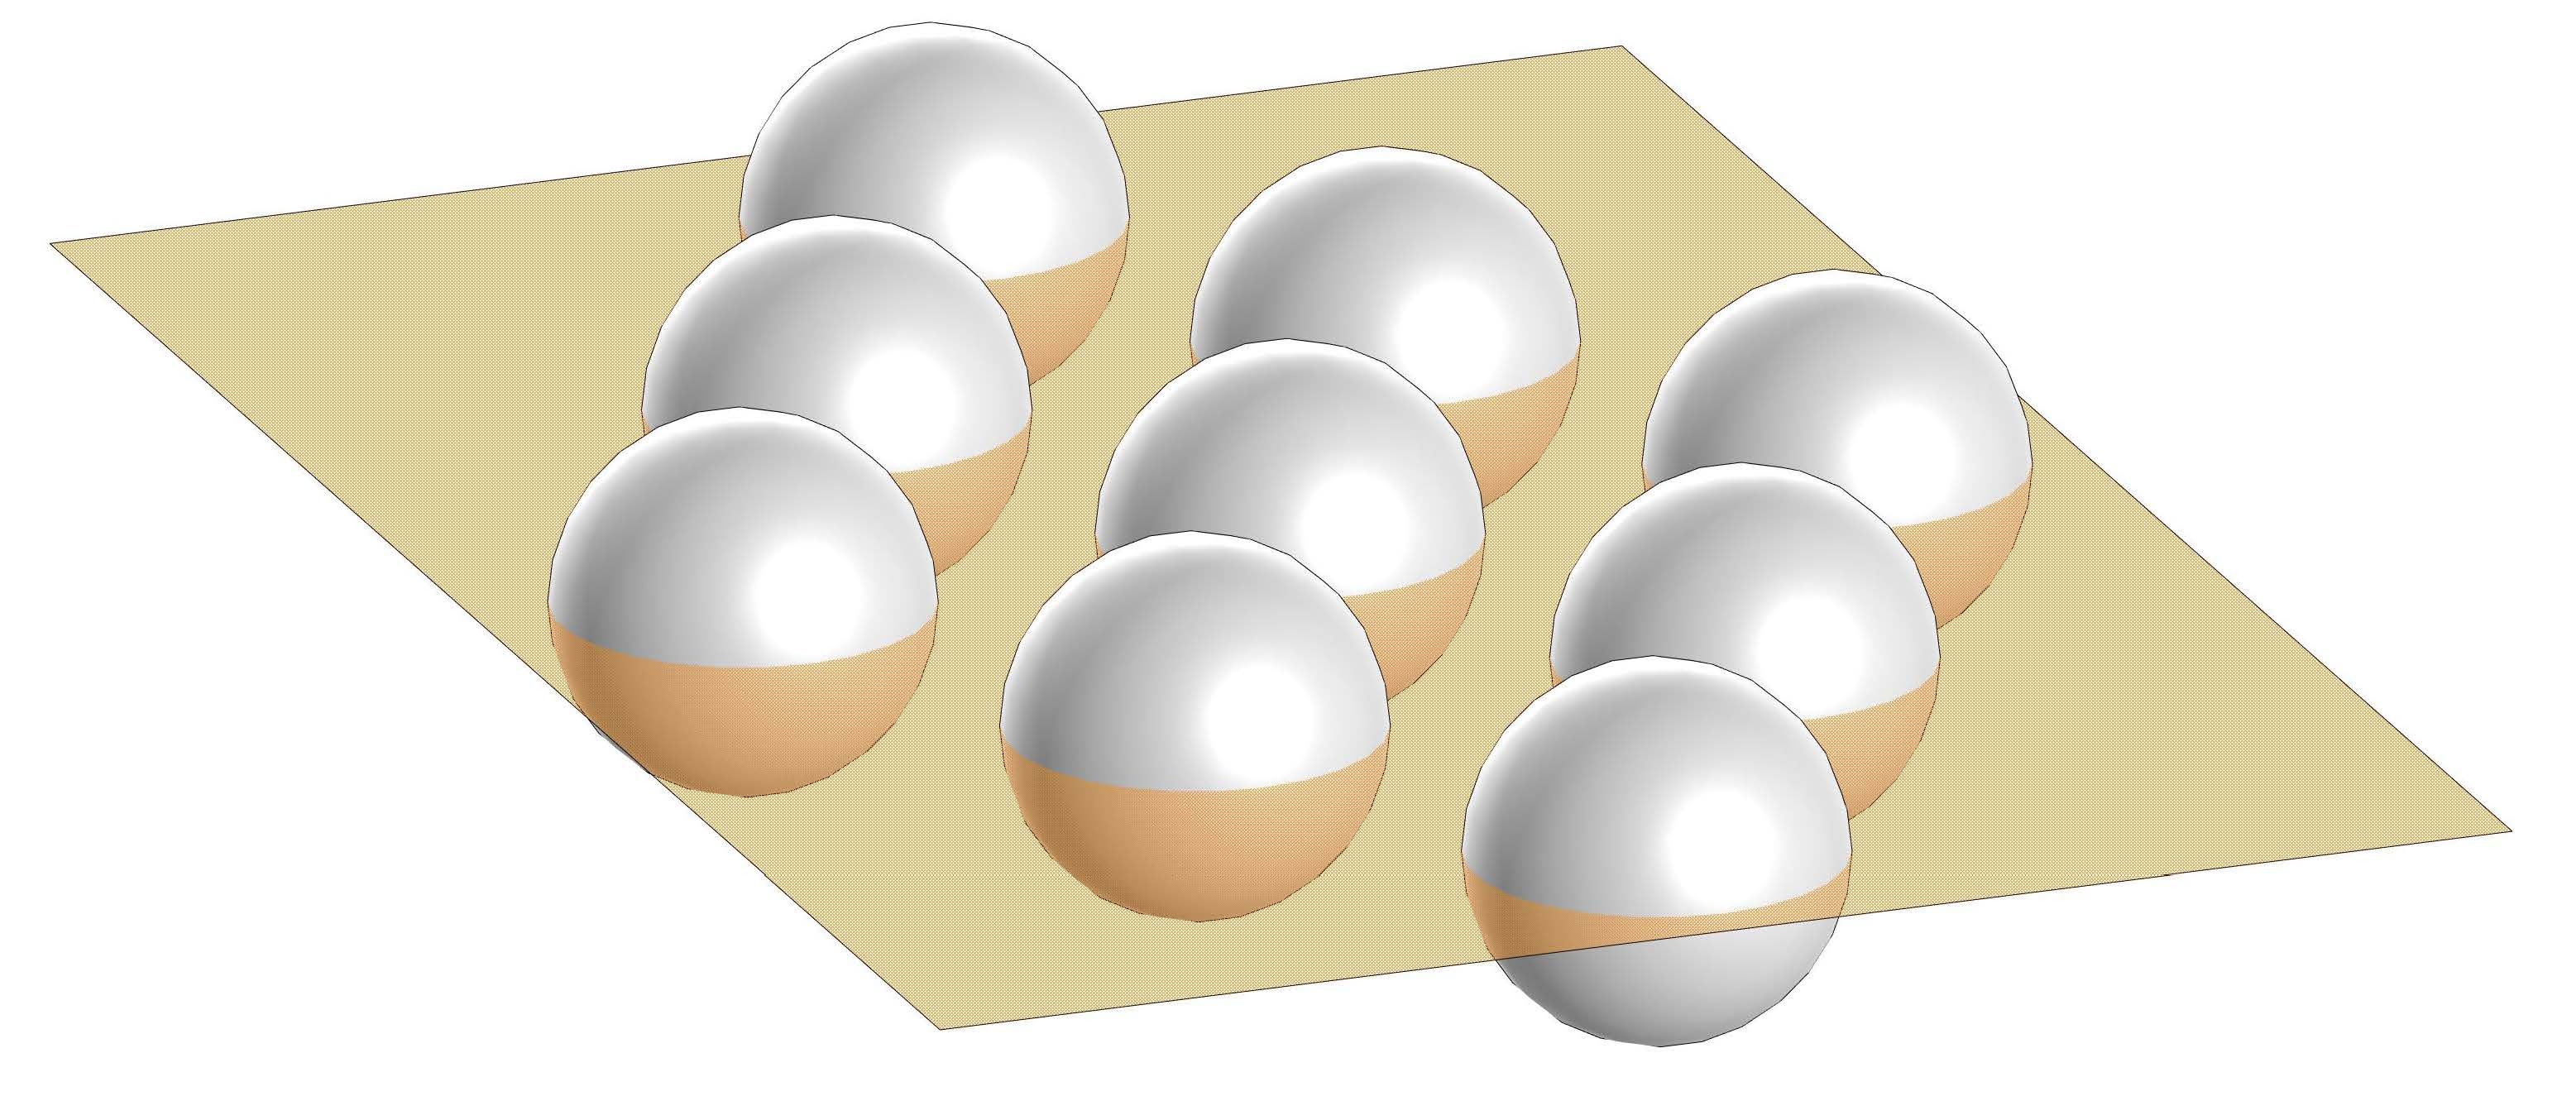
\includegraphics[width=0.45\textwidth]{images/a26.png}
\caption{Фрагмент распределения частиц относительно поверхности.}
\label{fig:surface_particles}
\end{figure}

\begin{figure}[h]
\centering
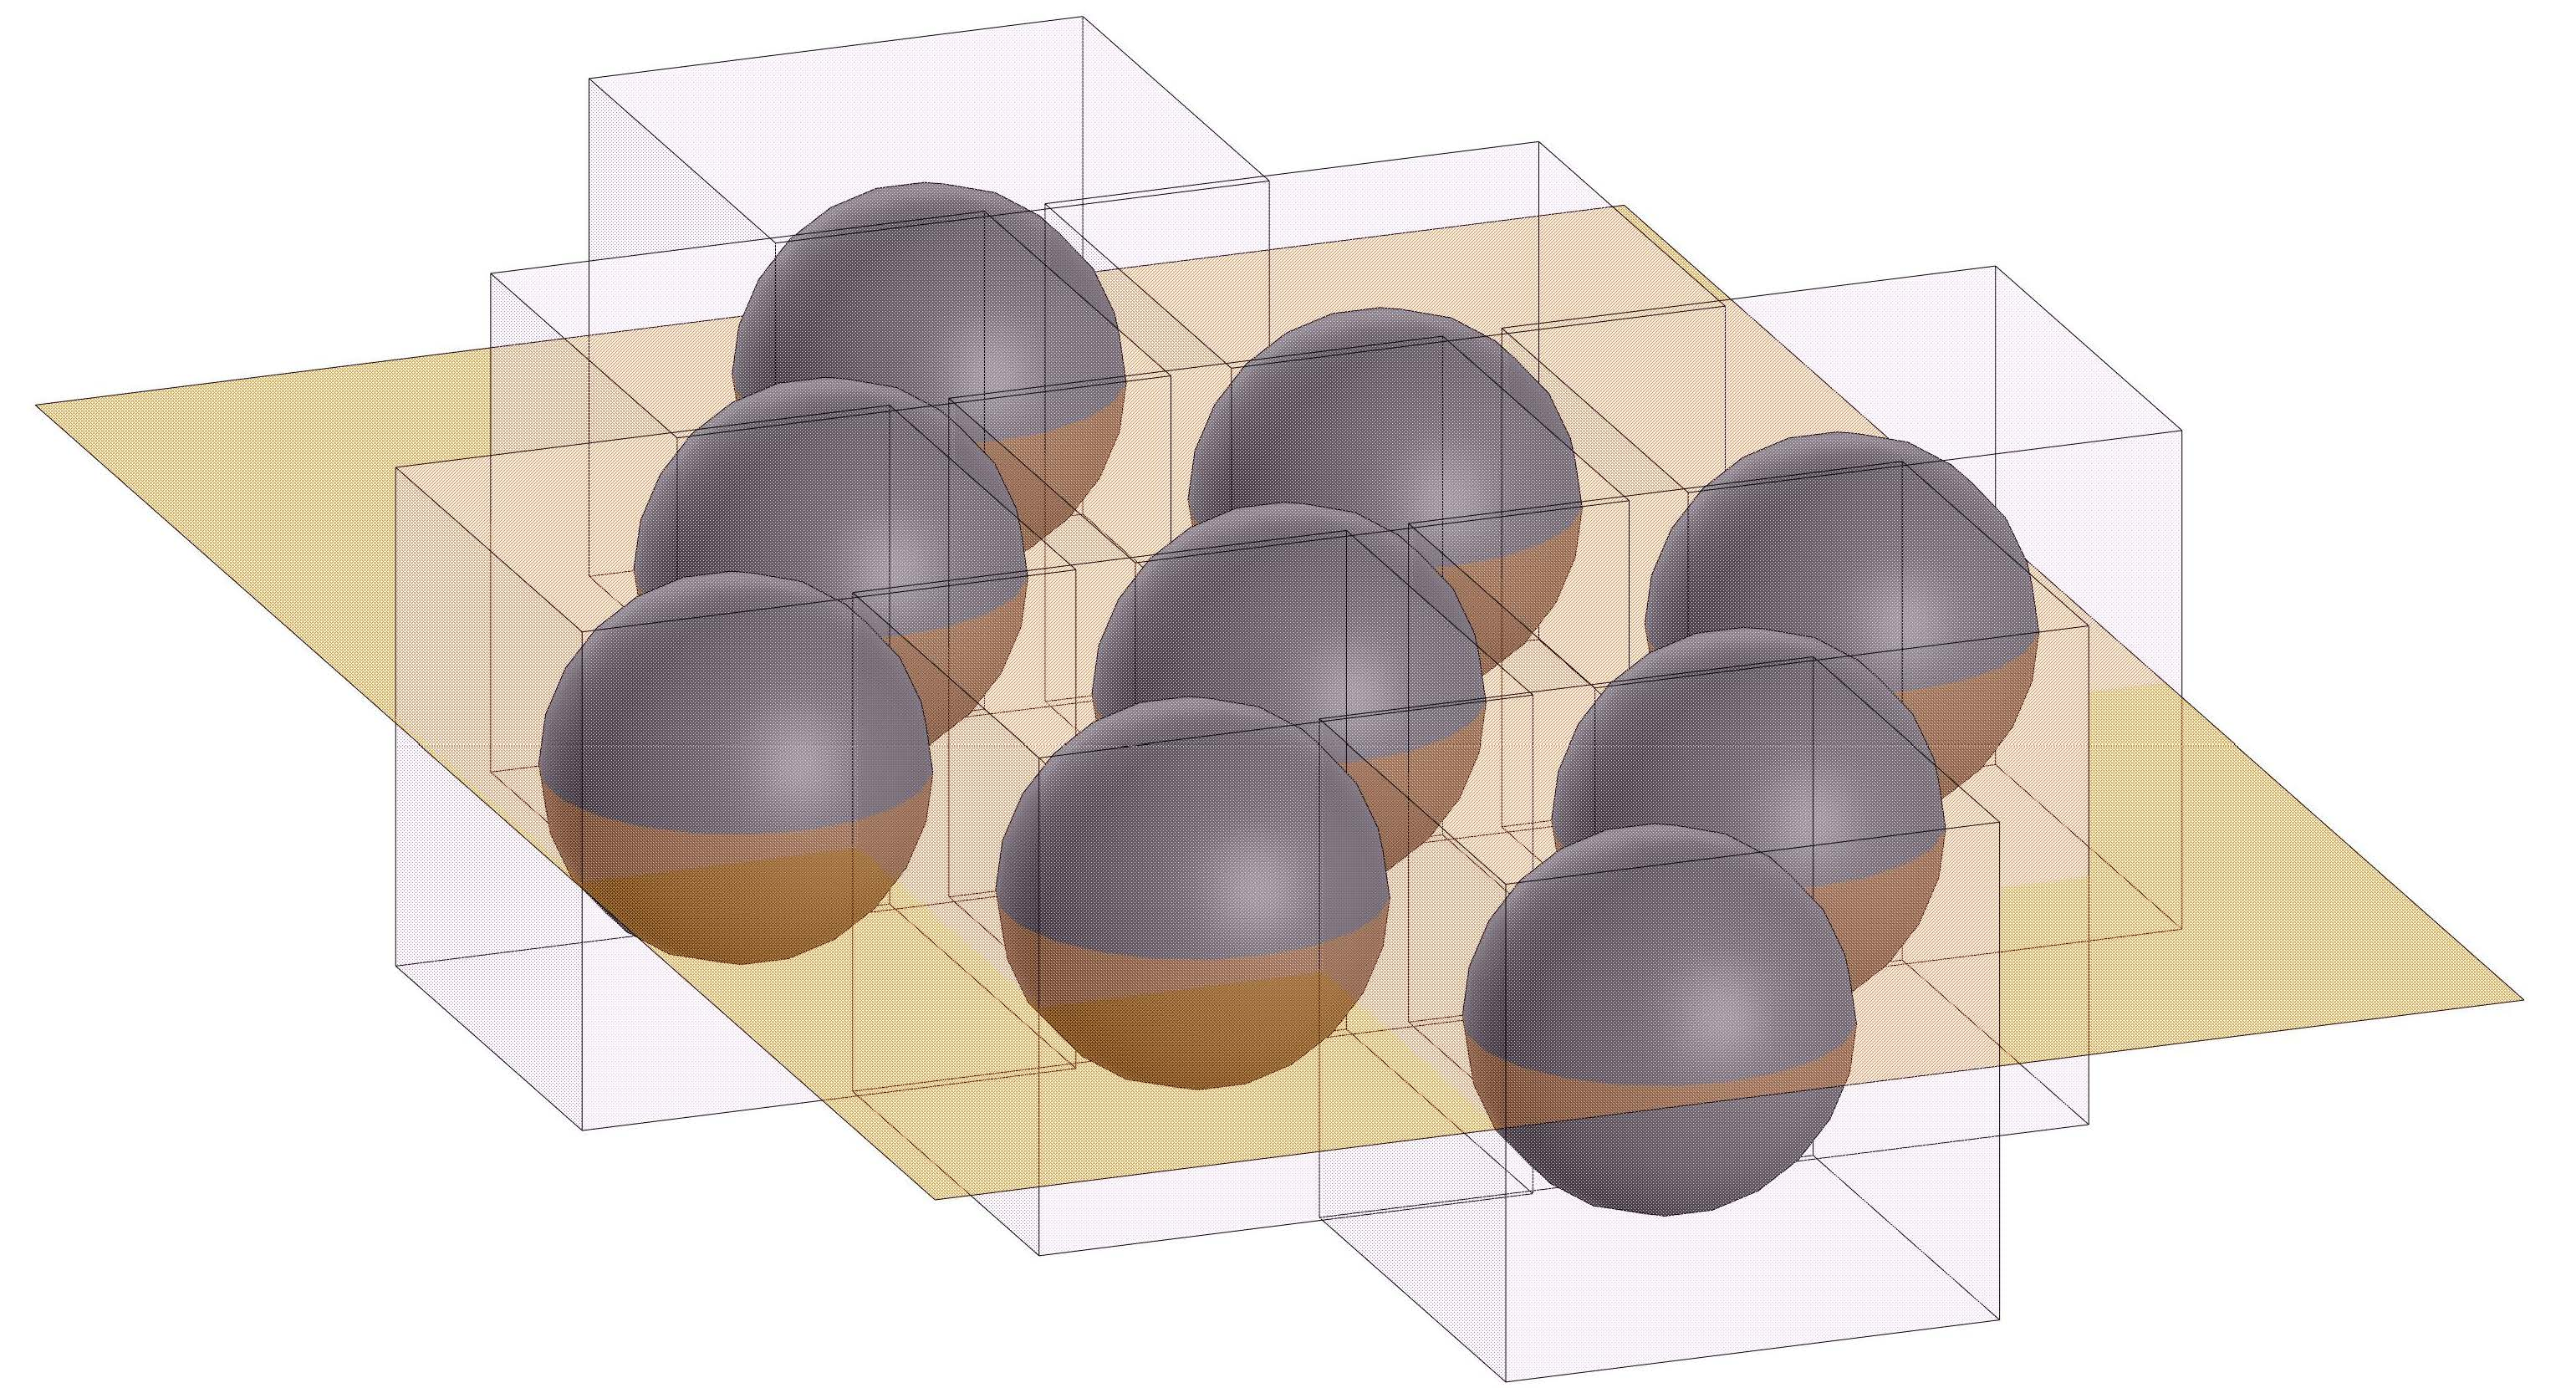
\includegraphics[width=0.45\textwidth]{images/a27.png}
\caption{Обитаемое пространство у поверхности.}
\label{fig:surface_habitat}
\end{figure}

Вывод о незначительности величины пространственного дрейфа частиц в Свободном эфире не позволяет применить проверенные методические подходы к решению задач кинетики, хорошо зарекомендовавшие себя применительно к газообразным средам, где атомы и молекулы представлены точками сосредоточения массы, а длина свободного пробега многократно превышает их размеры. В среде физического вакуума всё ровно наоборот. На рис. \ref{fig:surface_particles} представлен плоский фрагмент распределения частиц относительно рассматриваемой поверхности, где Амеры расположены в вершинах равносторонних треугольников с длиной стороны \(1,5\,d_a\), имитирующих грань тетраэдра. Рис. \ref{fig:surface_habitat} даёт представление об «обитаемом пространстве», в котором частицы эфира проводят своё «хаотическое» существование. Сталкиваясь, частицы блуждают в непосредственной близости от заданной поверхности, не теряя с ней «контакта» в виде той или иной степени пересечения. Ограничение возможности смещения частиц совершенно не ограничивает их возможность переносить через условную поверхность количество движения или импульс. Импульс частицы имеет направление и величину в каждый момент времени и изменяется в результате каждого акта соударения, при этом область изменения направления лежит в пределах телесного угла \(4\pi\), как изображено ранее на рис. \ref{fig:diagrams}. Нас интересует односторонний поток импульса, перпендикулярный плоской поверхности единичной площади, поэтому из всех возможных направлений вектора импульса частицы будем учитывать те, у которых ортогональная проекция \((\mathbf{v}_{\text{сэ}})_s\) на поверхность совпадает по направлению с вектором поверхности \(\mathbf{n}\), как изображено на рис. \ref{fig:flux}.

\begin{figure}[h]
\centering
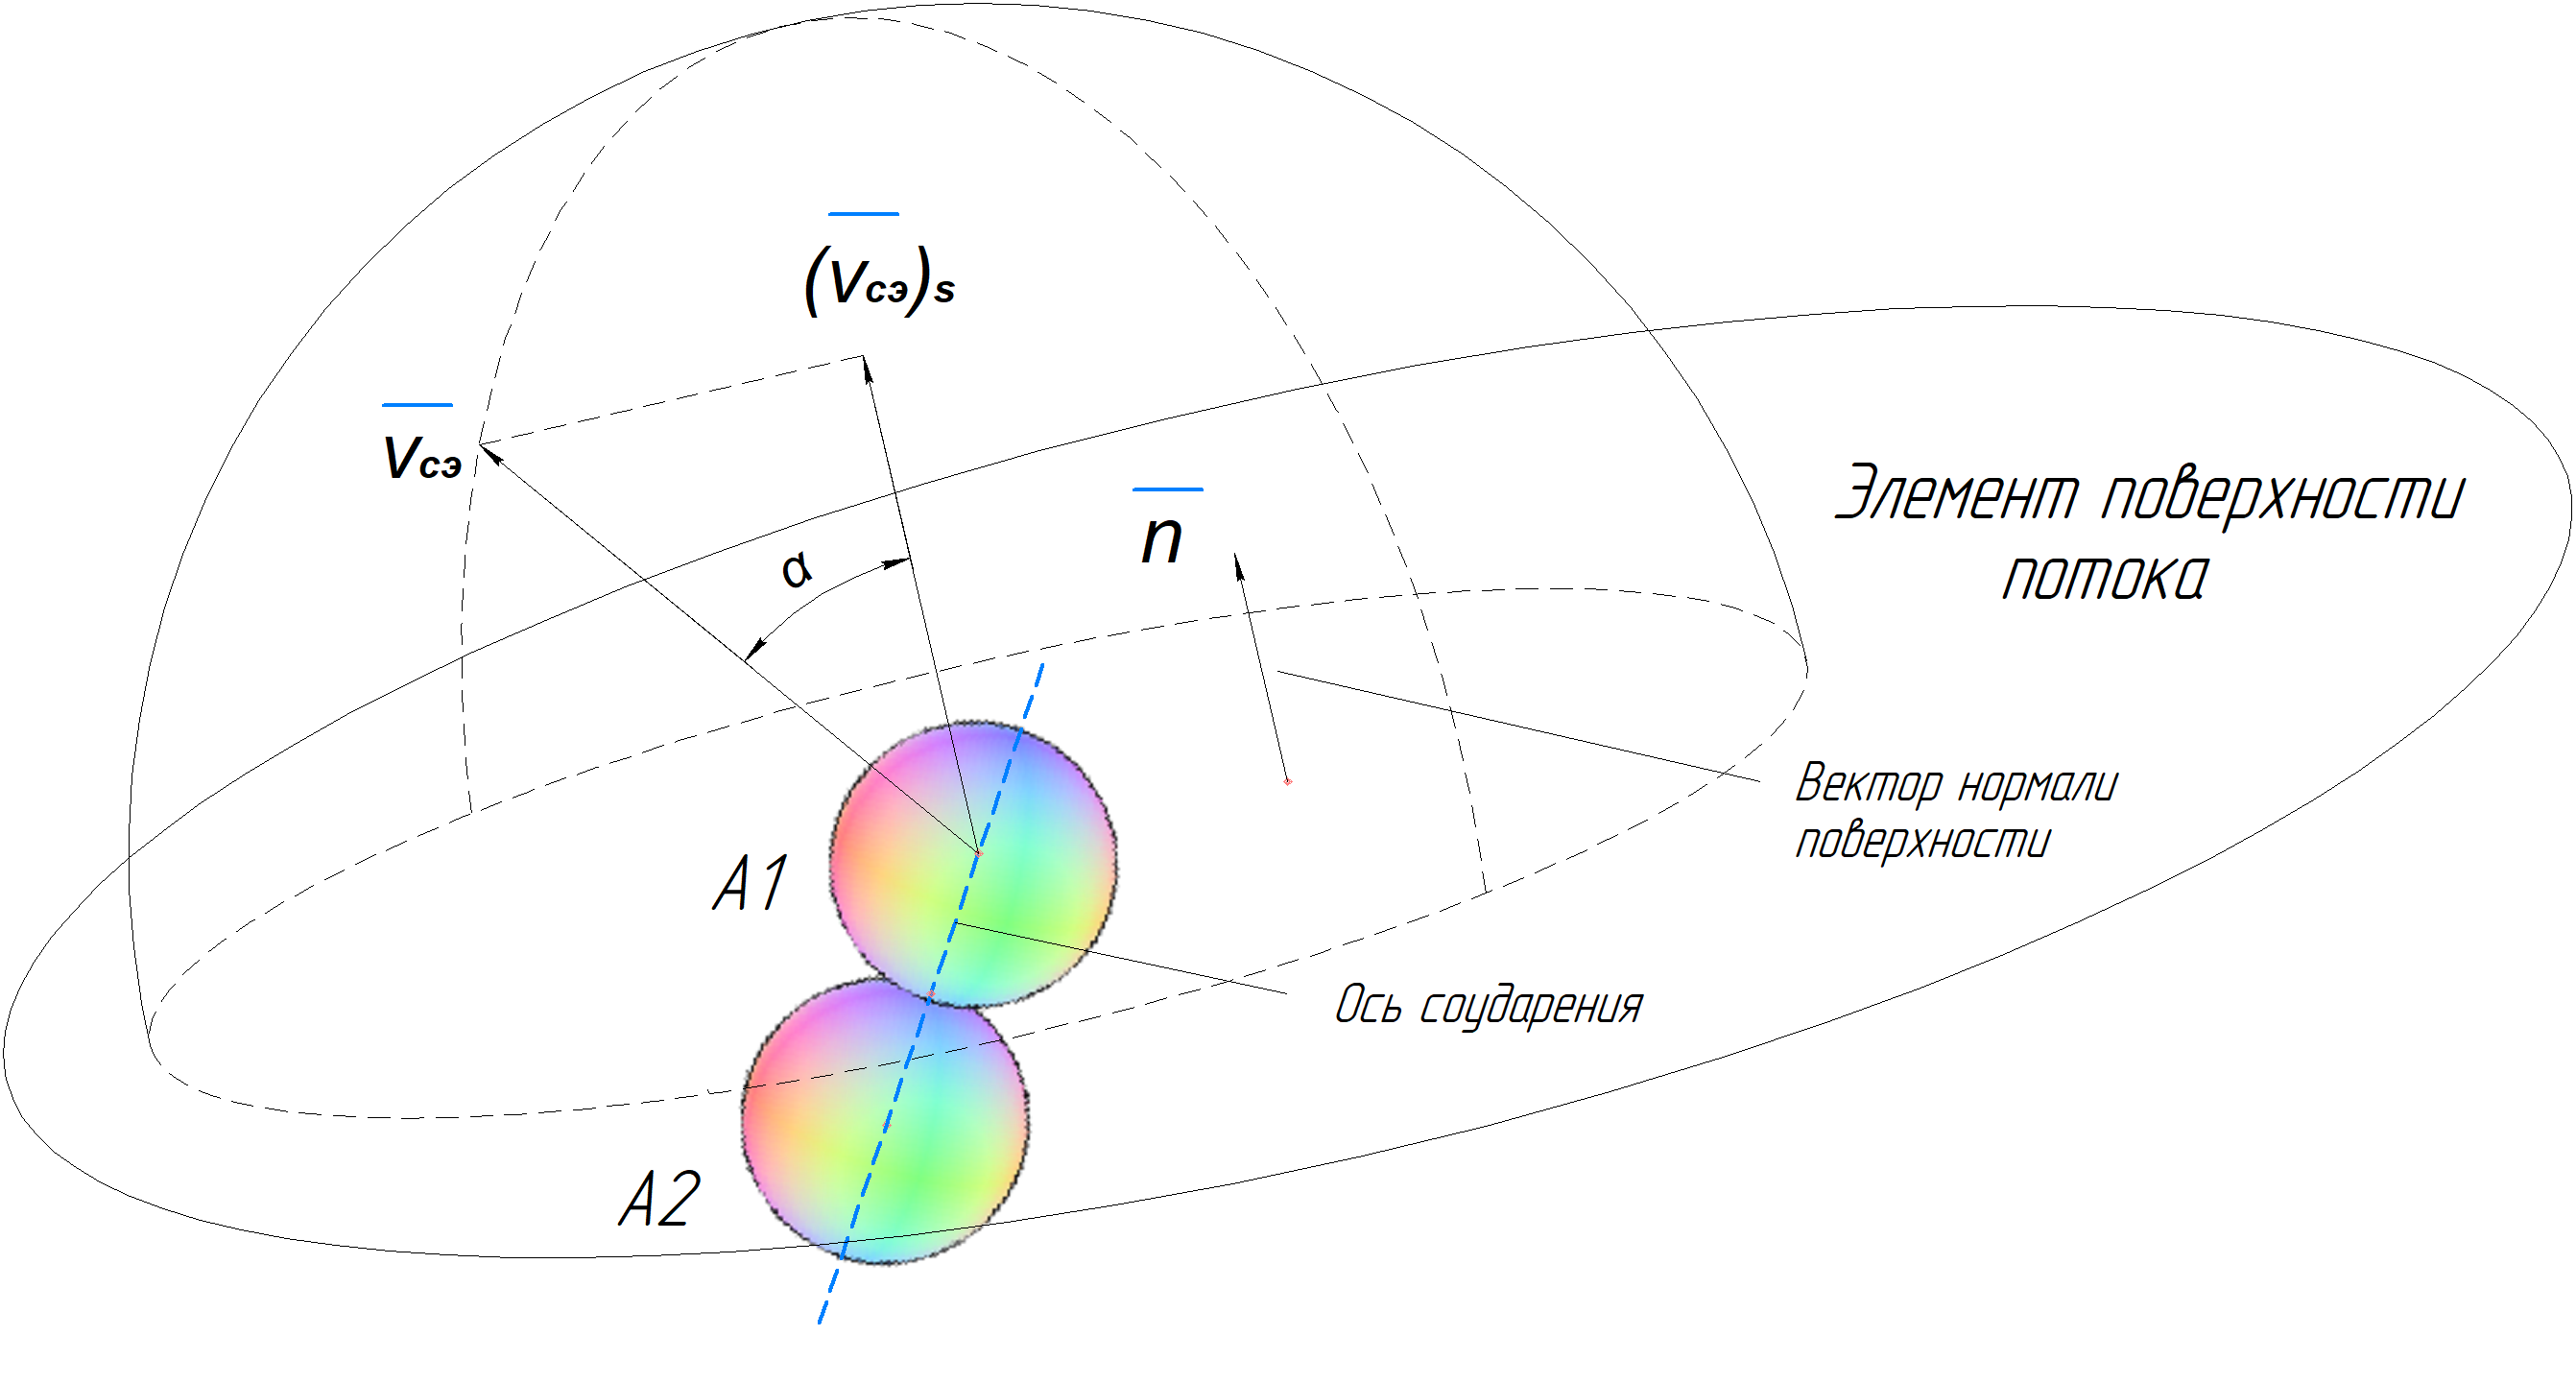
\includegraphics[width=0.7\textwidth]{images/a5.png}
\caption{К определению одностороннего потока импульса.}
\label{fig:flux}
\end{figure}

За единицу времени Амер свободного эфира испытывает \(\nu\) соударений, что при среднем значении скорости \(\|\mathbf{v}_{\text{сэ}}\|\), превышающем величину скорости света, составляет величину \(\nu = \frac{8\pi}{27 d_a}\|\mathbf{v}_{\text{сэ}}\| > 10^{30}\). Ровно столько раз изменяют своё направление и величину импульс каждой частицы Свободного эфира, а в силу его изотропности эти направления равновероятны в пределах телесного угла \(4\pi\), которому можно сопоставить соответствующую сферическую поверхность. Воспользуемся методикой, приведённой В.П. Поповым в учебнике «Диффузия» (М.: МФТИ, 2016), для одностороннего потока. В нашем случае хаотического движения частиц, изображённого на рис. \ref{fig:flux}, задача состоит в определении величины среднего значения \(\langle(\mathbf{v}_{\text{сэ}})_s\rangle\) за единицу времени применительно к Амеру \(A_1\). Амер \(A_2\) изображён для отображения акта столкновения и \textbf{оси соударения}, вдоль которой происходит соответствующий «обмен» компонентами импульса в точке касания частиц. Парность столкновений Амеров, как следует из рис. \ref{fig:flux}, предопределяет факт того, что при каждом последующем акте соударения проекция \((\mathbf{v}_{\text{сэ}})_s\) на направление вектора \(\mathbf{n}\) изменяет своё направление на противоположное. Случаями, когда \((\mathbf{v}_{\text{сэ}})_s\) ортогонально \(\mathbf{n}\), можно пренебречь ввиду их исчезающе малой вероятности. Изменение направления и величины импульса после каждого акта соударения не отменяет того, что согласно закону его сохранения, в том числе для абсолютно упругих столкновений:
\[
m_a(\mathbf{v}_{\text{сэ}})_{A1} + m_a(\mathbf{v}_{\text{сэ}})_{A2} = m_a(\mathbf{v}_{\text{сэ}})'_{A1} + m_a(\mathbf{v}_{\text{сэ}})'_{A2} \;\Longrightarrow\; \|(\mathbf{v}_{\text{сэ}})_{A1} + (\mathbf{v}_{\text{сэ}})_{A2}\| = \|(\mathbf{v}_{\text{сэ}})'_{A1} + (\mathbf{v}_{\text{сэ}})'_{A2}\|.
\]
Следовательно, допустимо предполагать, что вследствие большой величины частоты парных столкновений (более \(10^{30}\) соударений в секунду) величину скорости частиц свободного эфира можно положить равной среднему значению скорости \(\|\mathbf{v}_{\text{сэ}}\| = \langle\mathbf{v}_{\text{сэ}}\rangle\). Для одностороннего потока хаотически движущихся частиц справедливо равенство, которое применительно к нашей задаче выглядит \(\langle(\mathbf{v}_{\text{сэ}})_s\rangle = \frac{1}{2}\langle\mathbf{v}_{\text{сэ}}\rangle\), то есть \textbf{величина среднего значения скорости в направлении потока составляет половину от значения средней скорости движения частиц свободного эфира}. Для удобства далее будем считать \(\langle\mathbf{v}_{\text{сэ}}\rangle = v_{\text{сэ}}\). Таким образом, наша задача о направленном потоке импульса через произвольную выделенную плоскую поверхность ввиду особенности движения частиц сводится к суммированию числа импульсов одиночного Амера за единицу времени в нужном направлении с последующим суммированием по количеству частиц, «обитающих» на единице площади выделенной плоской поверхности:
\[
j_{\text{imp}} = \frac{1}{6} m_a v_{\text{сэ}}^2 n_{as} \nu = 0,3\, \frac{m_a v_{\text{сэ}}^2}{d_a^3} = \frac{12\pi}{27} n_{\text{сэ}} \varepsilon \approx 1,4\, n_{\text{сэ}} \varepsilon,
\]
где \(\varepsilon = \frac{1}{2} m_a v_{\text{сэ}}^2\) — среднее значение величины энергии движения Амера в свободном эфире, \(n_{as}\) — число Амеров на единице площади выделенной поверхности (поверхностная плотность частиц), \(\nu\) — число столкновений единичного Амера в единицу времени. По факту это уравнение представляет зависимость скорости изменения плотности потока импульса от кинетических и пространственных параметров частиц Свободного эфира. Уравнение записано в традиционной форме скорости молекулярной физики и термодинамики; при этом надо отметить, что скорость «передачи» импульса через поверхность единичной площади есть не что иное, как аналог давления для газообразной фазы существования весомой материи. Таким образом, полученное уравнение устанавливает связь давления Свободного эфира с кинетическими и пространственными параметрами его Амеров:
\[
p = 0,3\,\frac{m_a v_{\text{сэ}}^2}{d_a^3} = \frac{12\pi}{27} n_{\text{сэ}} \varepsilon \approx 1,4\, n_{\text{сэ}} \varepsilon.
\]
Для сравнения запишем аналогичное уравнение для идеального газа, где геометрические характеристики молекул газа в расчёт не принимаются:
\[
p = \frac{2}{3} n \varepsilon \approx 0,67\, n \varepsilon,
\]
где \(n\) — число молекул в единице объёма газа, \(\varepsilon\) — среднее значение кинетической энергии молекулы газа.
